\begin{pastexam}[label={px:gw3-109-ds-04}]{關務三等資訊處理 109 年 第四題}
（申論；20 分）

給予一串資料：45, 30, 40, 65, 68, 60, 70, 50，將此串資料依序建成一 max-heap 樹，並說明如何從此 max-heap 樹進行由小至大的排序（Sorting）。（20 分）
\end{pastexam}

\begin{pastsoln}
答案：max-heap 的陣列為 70, 65, 68, 50, 45, 40, 60, 30；堆積排序後得 30, 40, 45, 50, 60, 65, 68, 70。

「依序建成」理解成一個一個插入（放到最後再往上調整，資結書第~8.1~節）。 陣列索引從 $1$ 開始，$A[i]$ 的父節點是 $A[\lfloor i/2 \rfloor]$。

\textbf{建 max-heap}。
\begin{center}
\small
\begin{tabular}{lll}
\toprule
插入 & 往上調整 & 插入後的陣列 $A[1..]$ \\
\midrule
45 & 根 & 45 \\
30 & $30 \le 45$，不動 & 45, 30 \\
40 & $40 \le 45$，不動 & 45, 30, 40 \\
65 & 和 30 交換，再和 45 交換 & 65, 45, 40, 30 \\
68 & 和 45 交換，再和 65 交換 & 68, 65, 40, 30, 45 \\
60 & 和 40 交換，$60 \le 68$ 停 & 68, 65, 60, 30, 45, 40 \\
70 & 和 60 交換，再和 68 交換 & 70, 65, 68, 30, 45, 40, 60 \\
50 & 和 30 交換，$50 \le 65$ 停 & 70, 65, 68, 50, 45, 40, 60, 30 \\
\bottomrule
\end{tabular}
\end{center}
\begin{center}
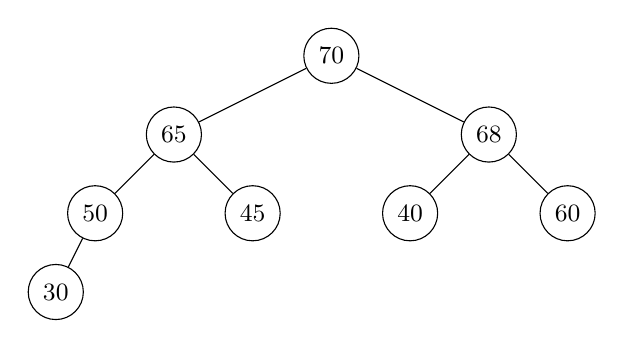
\begin{tikzpicture}[level distance=10mm,level 1/.style={sibling distance=40mm},level 2/.style={sibling distance=20mm},
  level 3/.style={sibling distance=10mm},every node/.style={circle,draw,minimum size=7mm,inner sep=0pt,font=\small}]
\node {70}
  child {node {65} child {node {50} child {node {30}} child[missing]} child {node {45}}}
  child {node {68} child {node {40}} child {node {60}}};
\end{tikzpicture}
\end{center}
檢查：每個節點都不小於子節點（$70 \ge 65, 68$；$65 \ge 50, 45$；$68 \ge 40, 60$；$50 \ge 30$）。 （若改用由下而上的 Build-Max-Heap，對原陣列
做下沉，結果是 $70, 68, 60, 65, 30, 45, 40, 50$，也是合法的 max-heap；題目說「依序」，用插入的版本。）

\textbf{由小到大排序：堆積排序}（資結書第~14.6~節，虛擬碼~14.13）。 max-heap 的根是最大值。 重複以下步驟，$n$ 從 $8$ 減到 $2$：把根 $A[1]$ 和最後一個
$A[n]$ 交換，最大值就放到它的最終位置 $A[n]$；堆積大小減一，再把新的根往下調整（和較大的子節點交換，直到不小於子節點），恢復 max-heap。
\begin{center}
\small
\begin{tabular}{cll}
\toprule
交換 & 調整後的堆積 & 已排好（陣列尾端） \\
\midrule
$70 \leftrightarrow 30$ & 68, 65, 60, 50, 45, 40, 30 & 70 \\
$68 \leftrightarrow 30$ & 65, 50, 60, 30, 45, 40 & 68, 70 \\
$65 \leftrightarrow 40$ & 60, 50, 40, 30, 45 & 65, 68, 70 \\
$60 \leftrightarrow 45$ & 50, 45, 40, 30 & 60, 65, 68, 70 \\
$50 \leftrightarrow 30$ & 45, 30, 40 & 50, 60, 65, 68, 70 \\
$45 \leftrightarrow 40$ & 40, 30 & 45, 50, 60, 65, 68, 70 \\
$40 \leftrightarrow 30$ & 30 & 40, 45, 50, 60, 65, 68, 70 \\
\bottomrule
\end{tabular}
\end{center}
例如第一列：30 換到根，子節點 65、68，和較大的 68 交換；30 的新子節點 40、60，和 60 交換；到葉，停。 最後陣列是
$30, 40, 45, 50, 60, 65, 68, 70$，由小到大。 用 max-heap 得到由小到大的結果，是因為每次把最大的放到陣列最後面。

時間：建堆積（逐一插入）$O(n \log n)$，每次取出並調整 $O(\log n)$、共 $n - 1$ 次，堆積排序總共 $O(n \log n)$，額外空間 $O(1)$，不穩定。
\end{pastsoln}
